%=========================================================
% SEMINAR REPORT
% REAL-TIME DETECTION METHOD FOR CRACKED EGGS BASED ON
% IMPROVED YOLOV8 AND DUAL VERIFICATION WITH TRIPLE
% CLASSIFICATION GRANULARITY
%=========================================================

\documentclass[12pt,a4paper]{report}
\usepackage[T1]{fontenc}
\usepackage[utf8]{inputenc}

%=========================================================
% PACKAGES
%=========================================================

\usepackage[a4paper,
            top=1in,
            bottom=1in,
            left=1.3in,
            right=1in]{geometry}

% PDFLaTeX-compatible Times-style font
\usepackage{newtxtext}
\usepackage{newtxmath}

\usepackage{graphicx}
\graphicspath{{./}{./figures/}}
\usepackage{fancyhdr}
\usepackage{titlesec}
\usepackage{tocloft}
\usepackage{setspace}
\usepackage{amsmath,amssymb}
\usepackage{enumitem}
\usepackage{hyperref}
\usepackage{booktabs}
\usepackage{array}
\usepackage{caption}
\usepackage{xcolor}
\usepackage{float}
\usepackage{ragged2e}
\usepackage[nottoc]{tocbibind}
\usepackage{longtable}

%=========================================================
% HYPERLINK SETTINGS
%=========================================================

\hypersetup{
    colorlinks=true,
    linkcolor=black,
    citecolor=black,
    urlcolor=blue,
    pdftitle={REAL-TIME DETECTION METHOD FOR CRACKED EGGS BASED ON IMPROVED YOLOV8 AND DUAL VERIFICATION WITH TRIPLE CLASSIFICATION GRANULARITY},
    pdfauthor={Arjun Manoj}
}

%=========================================================
% GENERAL FORMATTING
%=========================================================

\onehalfspacing
\fontsize{12}{18}\selectfont

\setlength{\parindent}{0.5in}
\setlength{\parskip}{0pt}

%=========================================================
% CHAPTER FORMATTING
%=========================================================

\titleformat{\chapter}[display]
    {\normalfont\fontsize{16}{19}\selectfont\bfseries\centering}
    {\chaptertitlename\ \thechapter}
    {14pt}
    {\fontsize{16}{19}\selectfont\centering}

\titlespacing*{\chapter}
    {0pt}
    {-8pt}
    {14pt}

%=========================================================
% SECTION FORMATTING (EXACT 14PT)
%=========================================================

\titleformat{\section}
    {\normalfont\fontsize{14}{17}\selectfont\bfseries}
    {\thesection}
    {0.5em}
    {}

\titleformat{\subsection}
    {\normalfont\fontsize{14}{17}\selectfont\bfseries}
    {\thesubsection}
    {0.5em}
    {}

%=========================================================
% TABLE OF CONTENTS FORMATTING
%=========================================================

\setlength{\cftbeforechapskip}{10pt}
\setlength{\cftbeforesecskip}{4pt}

\renewcommand{\cftchapfont}{\fontsize{12}{14}\selectfont\bfseries}
\renewcommand{\cftsecfont}{\fontsize{12}{14}\selectfont}

\renewcommand{\cftchappagefont}{\fontsize{12}{14}\selectfont\bfseries}
\renewcommand{\cftsecpagefont}{\fontsize{12}{14}\selectfont}

\renewcommand{\cfttoctitlefont}
    {\hfill\fontsize{14}{17}\selectfont\bfseries}

\renewcommand{\cftaftertoctitle}
    {\hfill}

%=========================================================
% HEADER AND FOOTER
%=========================================================

\pagestyle{fancy}

\fancyhf{}

\fancyhead[L]{
    \footnotesize College of Engineering, Cherthala
}

\fancyhead[R]{
    \footnotesize\leftmark
}

\fancyfoot[L]{
    \small Department of Computer Science and Engineering
}

\fancyfoot[R]{
    \small\thepage
}

\renewcommand{\headrulewidth}{0.4pt}
\renewcommand{\footrulewidth}{0.4pt}

\renewcommand{\chaptermark}[1]{
    \markboth{#1}{}
}

%=========================================================
% PLAIN PAGE STYLE
%=========================================================

\fancypagestyle{plain}{
    \fancyhf{}

    \fancyfoot[L]{
        \small Department of Computer Science and Engineering
    }

    \fancyfoot[R]{
        \small\thepage
    }

    \renewcommand{\headrulewidth}{0pt}
    \renewcommand{\footrulewidth}{0.4pt}
}

%=========================================================
% FIGURE AND TABLE CAPTION FORMAT
%=========================================================

\captionsetup[figure]{
    font=normalsize,
    labelfont=normalfont,
    justification=centering,
    singlelinecheck=true
}

\captionsetup[table]{
    font=normalsize,
    labelfont=bf,
    justification=centering,
    singlelinecheck=true
}

%=========================================================
% DOCUMENT INFORMATION
%=========================================================

\newcommand{\reporttitle}{REAL-TIME DETECTION METHOD FOR CRACKED EGGS BASED ON IMPROVED YOLOV8 AND DUAL VERIFICATION WITH TRIPLE CLASSIFICATION GRANULARITY}
\newcommand{\studentname}{ARJUN MANOJ}
\newcommand{\rollno}{CEC23CS043}
\newcommand{\guidename}{Mrs. NANDANA RAJ R}
\newcommand{\seminarmonth}{SEPTEMBER 2026}
\newcommand{\coordinator}{Mrs. Deepa C G}
\newcommand{\hodname}{Dr. Preetha Theresa Joy}
\newcommand{\principalname}{Dr. Jaya VL}

%=========================================================
% DOCUMENT
%=========================================================

\begin{document}

%=========================================================
% COVER PAGE
%=========================================================

\begin{titlepage}
\thispagestyle{empty}
\begin{center}

\vspace*{0.3cm}

{\Large\bfseries A SEMINAR REPORT ON}\par

\vspace{0.5cm}

{\fontsize{17}{21}\selectfont\bfseries
REAL-TIME DETECTION METHOD FOR CRACKED EGGS\\
BASED ON IMPROVED YOLOV8 AND DUAL VERIFICATION\\
WITH TRIPLE CLASSIFICATION GRANULARITY}\par

\vfill

{\large\itshape Submitted By}\par
\vspace{0.2cm}
{\large\bfseries\itshape \studentname\ (\rollno)}\par

\vfill

{\large\itshape under the esteemed guidance of}\par
\vspace{0.2cm}
{\large\bfseries\itshape \guidename}\par
\vspace{0.1cm}
{\large\itshape (Assistant Professor)}\par
\vspace{0.15cm}
{\large\itshape Department of Computer Science and Engineering}\par

\vfill


\includegraphics[width=3.2cm]{logo.jpg}\par

\vfill

{\large\bfseries \seminarmonth}\par
\vspace{0.05cm}
{\large\bfseries DEPARTMENT OF COMPUTER SCIENCE AND ENGINEERING}\par
{\large\bfseries COLLEGE OF ENGINEERING, PALLIPPURAM P O, CHERTHALA,}\par
{\large\bfseries ALAPPUZHA PIN: 688541,}\par
{\large\bfseries PHONE: 0478 2553416, FAX: 0478 2552714}\par
{\large\bfseries http://www.cectl.ac.in}\par

\vspace*{0.3cm}
\end{center}
\end{titlepage}

% =========================================================
% SECOND TITLE PAGE
% =========================================================

\begin{titlepage}
\thispagestyle{empty}
\begin{center}

\vspace*{0.2cm}

{\Large\bfseries A SEMINAR REPORT ON}\par

\vspace{0.45cm}

{\fontsize{16}{20}\selectfont\bfseries
REAL-TIME DETECTION METHOD FOR CRACKED EGGS\\
BASED ON IMPROVED YOLOV8 AND DUAL VERIFICATION\\
WITH TRIPLE CLASSIFICATION GRANULARITY}\par

\vspace{0.55cm}

{\large\itshape Submitted By}\par
\vspace{0.2cm}
{\large\bfseries\itshape \studentname\ (\rollno)}\par

\vspace{0.4cm}

{\large\itshape under the esteemed guidance of}\par
\vspace{0.2cm}
{\large\bfseries\itshape \guidename}\par
\vspace{0.1cm}
{\large\itshape (Assistant Professor)}\par

\vspace{0.4cm}

{\large\itshape In partial fulfillment of the requirements for the award of the degree}\par
{\large\itshape of}\par
{\large\bfseries Bachelor of Technology}\par
{\large\itshape in}\par
{\large\bfseries Computer Science and Engineering}\par
{\large\itshape of}\par
{\large\bfseries APJ Abdul Kalam Technological University}\par

\vfill


\includegraphics[width=3.2cm]{logo.jpg}\par

\vfill

{\large\bfseries \seminarmonth}\par
\vspace{0.05cm}
{\large\bfseries DEPARTMENT OF COMPUTER SCIENCE AND ENGINEERING}\par
{\large\bfseries COLLEGE OF ENGINEERING, PALLIPPURAM P O, CHERTHALA,}\par
{\large\bfseries ALAPPUZHA PIN: 688541,}\par
{\large\bfseries PHONE: 0478 2553416, FAX: 0478 2552714}\par
{\large\bfseries http://www.cectl.ac.in}\par

\vspace*{0.2cm}
\end{center}
\end{titlepage}

% =========================================================
% CERTIFICATE
% =========================================================

\thispagestyle{empty}
\begin{center}
{\large\bfseries DEPARTMENT OF COMPUTER SCIENCE AND ENGINEERING}\par
{\large\bfseries COLLEGE OF ENGINEERING CHERTHALA}\par
{\large\bfseries ALAPPUZHA-688541}\par
\vspace{0.3cm}

\includegraphics[width=2.8cm]{logo.jpg}\par
\vspace{0.3cm}
{\Large\bfseries C E R T I F I C A T E}\par
\end{center}

\vspace{0.5cm}
\noindent
This is to certify that, the seminar report titled \textbf{\textit{\reporttitle}} is a bonafide record of the \textbf{CSQ413 SEMINAR} presented by \textbf{\studentname\ (\rollno)}, Seventh Semester B.Tech. Computer Science \& Engineering student, under our guidance and supervision, in partial fulfillment of the requirements for the award of the degree B.Tech. Computer Science \& Engineering of APJ Abdul Kalam Technological University.

\vspace{1.2cm}
\begin{center}
\begin{tabular}{@{}c@{\hspace{0.45cm}}c@{\hspace{0.45cm}}c@{}}
\textbf{Guide} & \textbf{Co-ordinator} & \textbf{HoD}\\[0.75cm]

\parbox[c][0.55cm][c]{4.3cm}{\centering \guidename} &
\parbox[c][0.55cm][c]{4.3cm}{\centering \coordinator} &
\parbox[c][0.55cm][c]{4.3cm}{\centering \hodname}\\[0.25cm]

\parbox[c][0.45cm][c]{4.3cm}{\centering Assistant Professor} &
\parbox[c][0.45cm][c]{4.3cm}{\centering Assistant Professor} &
\parbox[c][0.45cm][c]{4.3cm}{\centering Professor}\\[0.25cm]

\parbox[c][1.35cm][c]{4.3cm}{\centering \small Dept. of Computer Science} &
\parbox[c][1.35cm][c]{4.3cm}{\centering \small Dept. of Computer Science} &
\parbox[c][1.35cm][c]{4.3cm}{\centering \small Dept. of Computer Science}

\end{tabular}
\end{center}

\newpage

% =========================================================
% ACKNOWLEDGEMENT
% =========================================================

\chapter*{ACKNOWLEDGEMENT}
This seminar work would not have been possible without the support and encouragement of many people. First and foremost, I give thanks to Almighty God who gave me the strength, resources and ability to complete the seminar successfully.

I would like to express my sincere gratitude to our Principal, \textbf{\principalname}, for providing the necessary facilities and support for the completion and presentation of this seminar.

I am also deeply grateful to the Head of the Department, \textbf{\hodname}, for her encouragement and support throughout the seminar work.

I extend my heartfelt thanks to my seminar co-ordinator, \textbf{\coordinator},\\\textbf{Mrs.~Seethamol~S} and \textbf{Mrs.~Vidya~S~Mony}, Assistant Professors, Department of Computer Science and Engineering, for their valuable coordination and guidance. I am especially grateful to my guide, \textbf{\guidename}, Assistant Professor, Department of Computer Science and Engineering, for her constant guidance, encouragement and constructive suggestions throughout this seminar.

I would also like to thank my dear friends for their cooperation and encouragement throughout the seminar. Their support and understanding made the completion of this work easier and more meaningful.

\newpage

%=========================================================
% ABSTRACT
%=========================================================

\chapter*{ABSTRACT}

\addcontentsline{toc}{chapter}{Abstract}

Eggshell integrity is a vital commercial quality indicator in the poultry processing industry. Approximately 3\% of fresh eggs suffer shell damage during production, handling, packaging and transit. Defective shells facilitate rapid bacterial penetration by pathogens such as \textit{Salmonella}, lead to internal moisture loss, cause liquid leakage and inflict substantial financial losses on poultry producers. Conventional sorting relies heavily on manual visual inspection, which is labor-intensive, subjective and vulnerable to worker visual fatigue. Non-destructive acoustic and traditional vision techniques struggle on dynamic conveyor lines due to factory acoustic noise, fluctuating illumination and natural dirt on unwashed eggs. Furthermore, conventional conveyors lack egg rotation mechanisms, leaving bottom surfaces uninspected.

This seminar presents an industrial-grade, real-time online detection method for cracked eggs based on an improved YOLOv8 framework and a dual verification mechanism with triple classification granularity. The mechanical conveying system integrates motor-driven rotating rollers across six parallel channels (360 eggs/minute throughput), rotating eggs through 360 degrees beneath an industrial CCD camera and uniform LED lighting box. Instead of binary classification, the framework introduces triple classification granularity: Category 1 (Intact Egg), Category 2 (Cracked Egg) and Category 3 (Crack Region). A redundant dual verification rule identifies an egg as damaged whenever either the overall cracked egg or localized crack region detector fires.

At the network architectural level, the baseline YOLOv8 model is structurally optimized for irregular hairline cracks. Deformable Convolution v2 (DCNv2) modules are integrated into the backbone to adapt receptive field shapes to jagged crack paths. A Weighted Bidirectional Feature Pyramid Network (BiFPN) replaces the standard PANet neck for multi-scale feature fusion. A dedicated P2 small target detection head operating on a $160 \times 160$ feature map is introduced to preserve micro-crack cues, while the Wise-IoU v2 (WIoUv2) loss function dynamically balances gradients across bounding box candidates. Experimental evaluations demonstrate that the improved YOLOv8 model achieves an mAP@0.5 of 92.9\% on the test set, representing a 5.2\% improvement over baseline YOLOv8 and outperforming Faster R-CNN, YOLOv5 and YOLOv11. On an industrial egg conveyor, the deployed system operates at 45 frames per second with an intact egg false alarm rate of 2.18\% and a compound broken egg miss rate of only 1.06\%, fully meeting industrial online grading criteria.

\clearpage

%=========================================================
% TABLE OF CONTENTS
%=========================================================

\pagenumbering{roman}

\tableofcontents

\clearpage

%=========================================================
% LIST OF FIGURES
%=========================================================

\listoffigures

\clearpage

%=========================================================
% LIST OF TABLES
%=========================================================

\listoftables

\clearpage

%=========================================================
% MAIN CONTENT
%=========================================================

\pagenumbering{arabic}
%=========================================================
% CHAPTER 1
%=========================================================

\chapter{Introduction}

\section{Background and Commercial Significance}

Table eggs represent one of the most widely consumed, nutrient-dense and economical sources of animal protein globally. With the growth of modern intensive poultry farming, egg production has expanded into an automated, high-throughput industrial sector. Modern commercial egg packaging facilities routinely process hundreds of thousands of eggs daily. In these high-capacity operations, preserving the physical integrity of the eggshell is of paramount importance to ensure food safety, extend product shelf life and protect commercial profitability.

The avian eggshell is a naturally engineered bioceramic composite structure composed predominantly of calcium carbonate (around 95\% to 97\% calcite crystal matrix) interwoven with an organic protein matrix and sealed by an outermost waxy cuticle layer. Despite possessing impressive mechanical compression strength along its major axis, the eggshell is inherently thin and brittle, making it susceptible to fracture when subjected to dynamic mechanical impacts, point stresses, vibrations and lateral compression during gathering, packing and transit.

Maintaining shell integrity constitutes the primary biological barrier preventing external microorganisms from invading the nutrient-rich interior of the egg. When the structural continuity of the shell is compromised, the commercial and hygienic value of the egg declines drastically. Developing fast, automated and non-destructive quality evaluation systems capable of detecting shell defects in real time has emerged as an urgent priority for modern agricultural engineering.

\section{Eggshell Integrity and Breakage Challenges}

Across commercial egg production and distribution pipelines, empirical surveys indicate that approximately 3\% of all fresh eggs suffer shell breakage prior to retail delivery. While this percentage may appear modest in isolation, its cumulative impact across facilities processing hundreds of thousands of eggs per day translates into massive economic losses annually for industrial egg producers.

The consequences of cracked eggshells are severe:
\begin{enumerate}[label=\arabic*.]

    \item \textbf{Pathogen Infiltration and Food Safety Hazards:} A hairline fissure ruptures the physical protection provided by the shell and underlying testaceous membranes. This fissure provides an open entry corridor for environmental bacteria, including dangerous foodborne pathogens such as \textit{Salmonella enteritidis} and \textit{Escherichia coli}, presenting severe health risks to consumers.

    \item \textbf{Loss of Internal Freshness and Spoilage:} The crack accelerates evaporation of internal moisture and dissipation of carbon dioxide, thinning the thick albumen, flattening the yolk and precipitating premature spoilage.

    \item \textbf{Leakage and Secondary Batch Contamination:} In automated grading and packaging machinery, cracked eggs frequently rupture under mechanical handling. Liquid albumen and yolk leak onto conveyor rollers and surrounding intact eggs, fouling sorting machinery and contaminating entire batches of clean, marketable eggs.

\end{enumerate}

\section{Limitations of Existing Inspection Modalities}

Historically, the identification of defective eggs has relied on manual visual inspection (manual candling), where trained workers visually observe eggs rolling over an illuminated light table. However, manual candling exhibits severe operational bottlenecks: extreme visual fatigue leading to declining accuracy after 20 to 30 minutes, subjective assessment, high labor costs and an inability to keep pace with modern conveyors processing over 360 eggs per minute.

To eliminate dependence on human labor, automated non-destructive detection technologies have been investigated:
\begin{itemize}

    \item \textbf{Acoustic Resonance Methods:} Mechanical strikers tap the eggshell to capture acoustic vibrational response spectra. While effective in quiet laboratories, acoustic methods are vulnerable to severe ambient acoustic noise from factory conveyors and mechanical contact risks micro-fracturing thin shells.

    \item \textbf{Traditional Computer Vision:} Classical algorithms employ grayscale thresholding (Otsu binarization) and edge filters. However, these methods fail on unwashed eggs where natural dust, feathers and dried manure streaks generate false edges that confuse thresholding rules.

    \item \textbf{Existing Deep Learning Approaches:} Prior convolutional networks (such as Faster R-CNN) suffer from excessive latency ($\le 17$ FPS) that fails to meet production speeds ($\ge 30$ FPS). Crucially, existing vision rigs lack egg rotation mechanisms, capturing only a single perspective and leaving the underside shell surface uninspected.

\end{itemize}

\section{Problem Statement}

Industrial egg processing facilities require an automated, real-time and non-destructive quality evaluation system capable of operating directly on high-speed conveyors carrying unwashed, moving eggs under actual factory conditions. The system must inspect the complete 360-degree surface of every egg to eliminate blind spots, operate at frame rates exceeding 30 frames per second (FPS) and maintain near-zero false negative rates for cracked eggs while minimizing false alarms on intact eggs carrying natural surface stains.

\section{Objectives}

The primary objective of this seminar study is to investigate, analyze and evaluate an industrial-grade, real-time cracked egg detection methodology based on an improved YOLOv8 architecture and a dual verification mechanism with triple classification granularity.

The specific objectives are:
\begin{enumerate}[label=\arabic*.]
    \item To examine a multi-channel conveying device with rotating rollers that enables complete 360-degree surface image acquisition without blind spots.
    \item To analyze the construction of an industrial dataset of unwashed eggs collected under dynamic production line conditions.
    \item To investigate the triple classification granularity scheme (Intact Egg, Cracked Egg and Crack Region) for multi-scale supervision.
    \item To study the structural enhancements incorporated into YOLOv8, including DCNv2, BiFPN, a P2 small target detection head and Wise-IoU v2 loss.
    \item To formulate the redundant dual verification decision logic and evaluate its mathematical efficacy in minimizing compound miss rates.
    \item To evaluate model performance through ablation experiments, benchmarks and live industrial conveyor line deployment.
\end{enumerate}

\section{Scope of the Report}

The scope of this report covers the mechanical conveying design, optical acquisition setup, convolutional neural network architecture, dynamic loss formulation, ablation studies and factory production line deployment proposed by Sun et al. (2026). The experimental analysis is grounded on a dynamic production dataset of 3,222 unwashed egg images from Guangzhou Suiping Enterprise Co., Ltd., benchmarked within a standardized PyTorch environment on an NVIDIA GeForce RTX 3060 hardware platform.

The remainder of this report is organized as follows: Chapter 2 details theoretical fundamentals of eggshell morphology, YOLOv8, DCNv2, BiFPN and loss functions; Chapter 3 reviews related literature; Chapter 4 presents the proposed methodology; Chapter 5 examines results and ablation findings; Chapter 6 discusses practical applications and deployment; and Chapter 7 outlines conclusions and future scope.
%=========================================================
% CHAPTER 2
%=========================================================

\chapter{Fundamentals}

\section{Eggshell Morphology and Defect Manifestation}

The avian eggshell is a specialized biological ceramic composite structure composed of approximately 95\% to 97\% crystalline calcium carbonate (calcite) embedded in an organic protein matrix. Morphologically, the shell consists of the inner and outer testaceous membranes, the mammillary layer, the palisade layer of columnar calcite crystals, the vertical crystal layer and the protective waxy cuticle. While the palisade layer imparts high compressive strength, the brittle calcite matrix is vulnerable to flexural tensile stresses and fracture propagation under localized impacts.

Eggshell defects manifest in several morphologies:
\begin{itemize}
    \item \textbf{Hairline Micro-Cracks:} Fine, narrow fissures with widths under 0.1 mm penetrating the calcite layer. Due to their minute aperture, they produce minimal optical shadow and subtle gradient transitions.
    \item \textbf{Impact and Puncture Cracks:} Fractures caused by sharp point contact, featuring a central crushed indentation surrounded by radiating star-like micro-fissures.
    \item \textbf{Reticular Spider-Web Cracks:} Intricate networks of interconnected fine cracks covering broad areas of the egg equator.
\end{itemize}

A critical challenge in automated vision is distinguishing genuine hairline cracks from non-defective surface artifacts present on unwashed eggs, such as pigmentation speckles, dust particles, feather residues and dried manure streaks.

\section{Object Detection and the YOLOv8 Architecture}

Object detection requires simultaneously classifying objects and predicting their spatial bounding boxes. Modern deep detectors are categorized into two-stage and single-stage frameworks:
\begin{itemize}
    \item \textbf{Two-Stage Detectors (e.g., Faster R-CNN):} Utilize a Region Proposal Network (RPN) followed by RoI pooling. While accurate, their multi-stage pipeline introduces substantial latency (10 to 18 FPS), precluding high-speed conveyor sorting.
    \item \textbf{Single-Stage Detectors (e.g., YOLO):} Frame detection as a single-pass regression problem, predicting bounding boxes and class probabilities simultaneously across a spatial grid.
\end{itemize}

YOLOv8 represents a modern state-of-the-art single-stage detector. Its architecture features a CSPDarknet backbone with C2f (Cross Stage Partial with two convolutions) modules, an SPPF (Spatial Pyramid Pooling Fast) pooling block and an anchor-free decoupled detection head that separates classification from bounding box regression. This anchor-free design eliminates manual anchor tuning and improves adaptation to objects of arbitrary aspect ratios.

\section{Deformable Convolutional Networks (DCNv2)}

Standard 2D convolution operates over a fixed regular sampling grid. For input feature map $X$ and kernel weights $w_k$, output $Y$ at coordinate $q$ is formalized as:
\begin{equation}
Y(q) = \sum_{k=1}^{K} w_k X(q + q_k)
\end{equation}
where $K$ is the kernel size (for $3 \times 3$, $K=9$) and $q_k$ represents fixed regular grid offsets. This rigid structure cannot conform to winding, irregular crack paths, causing sampling points to fall onto healthy shell regions.

Deformable Convolution v2 (DCNv2) breaks this limitation by adding learnable 2D spatial coordinate offsets $\Delta q_k$ and dynamic feature modulation scalars $\Delta m_k \in [0, 1]$:
\begin{equation}
Y(q) = \sum_{k=1}^{K} w_k X(q + q_k + \Delta q_k) \Delta m_k
\end{equation}
where $\Delta q_k$ dynamically reshapes the receptive field along the winding crack contour and $\Delta m_k$ modulates feature amplitude, suppressing non-crack shell textures.

\section{Multi-Scale Feature Fusion and BiFPN}

Feature Pyramid Networks resolve the trade-off between shallow spatial resolution and deep semantic abstraction. The baseline YOLOv8 utilizes PANet, which aggregates features using top-down and bottom-up pathways with equal weights.

The Weighted Bidirectional Feature Pyramid Network (BiFPN) improves multi-scale fusion by eliminating single-edge nodes, introducing cross-scale residual skip connections and applying fast normalized weighted fusion:
\begin{equation}
O = \sum_{i} \frac{w_i}{\epsilon + \sum_{j} w_j} \cdot I_i
\end{equation}
where $I_i$ is the input feature map at scale $i$, $w_i \ge 0$ is a learnable weight and $\epsilon = 0.0001$ ensures numerical stability. BiFPN dynamically balances shallow spatial details with deep semantics, enhancing resilience to shifting illumination.

\section{P2 Small Target Detection Head}

Baseline YOLOv8 downsamples input images ($640 \times 640$) by a factor of 32, generating detection heads at $80 \times 80$ (P3), $40 \times 40$ (P4) and $20 \times 20$ (P5). The smallest P3 head possesses an $8 \times 8$ pixel receptive field. Micro-cracks spanning fewer than 8 pixels lose high-frequency textural cues during downsampling.

Integrating an additional P2 small target detection head operating on a $160 \times 160$ feature map (stride 4, $4 \times 4$ pixel receptive field) preserves early-stage spatial gradients, dramatically boosting sensitivity to minute hairline fractures.

\section{Wise-IoU v2 Dynamic Loss Function}

Conventional bounding box regression losses (such as CIoU) enforce static penalties that disproportionately penalize low-quality outlier samples. Wise-IoU v2 (WIoUv2) introduces a dynamic non-monotonic focusing mechanism governed by the outlier degree $\beta$:
\begin{equation}
\beta = \frac{L_{\text{IoU}}}{\overline{L_{\text{IoU}}}} \in [0, +\infty)
\end{equation}
where $\overline{L_{\text{IoU}}}$ is the running moving average of the IoU loss.

The WIoUv2 loss is formalized as:
\begin{equation}
L_{\text{WIoUv2}} = L_{\text{IoU}}^{\gamma*} L_{\text{WIoUv1}}, \quad \gamma > 0
\end{equation}
where $L_{\text{IoU}}^{\gamma*} = (L_{\text{IoU}} / \overline{L_{\text{IoU}}})^\gamma$ serves as the dynamic non-monotonic focusing factor and $L_{\text{WIoUv1}}$ incorporates center distance penalties. WIoUv2 reduces gradient penalties on extreme outliers while focusing updates on moderately challenging samples.

\section{Dual Verification and Multi-Granularity Decision Theory}

Binary classification (intact versus cracked) suffers from single-point failure: a subtle crack that misses the global threshold results in an undetected broken egg. The proposed framework establishes triple classification granularity:
\begin{itemize}
    \item \textbf{Category 1 (Intact Egg):} Holistic undamaged egg body.
    \item \textbf{Category 2 (Cracked Egg):} Holistic egg body displaying shell rupture.
    \item \textbf{Category 3 (Crack Region):} Tightly bounded localized fracture zone.
\end{itemize}

Under dual verification logic, an egg is declared damaged if Category 2 OR Category 3 is detected. Assuming the error rates of the macro-scale classifier ($P(\text{Miss}_{\text{Egg}})$) and region detector ($P(\text{Miss}_{\text{Region}})$) are statistically decoupled, the compound miss probability is:
\begin{equation}
P(\text{Miss}_{\text{Overall}}) = P(\text{Miss}_{\text{Egg}}) \times P(\text{Miss}_{\text{Region}})
\end{equation}
This product drives compound defect escape rates down by an order of magnitude.
%=========================================================
% CHAPTER 3
%=========================================================

\chapter{Literature Survey}

\section{Traditional Acoustic and Optical Methods}

Automated quality inspection of eggshells has evolved through acoustic and optical processing techniques. Sun et al. (2020) investigated acoustic resonance inspection for hen and duck eggs using correlation analysis of impact sound waves. While intact shells displayed symmetric resonant peaks, factory background noise and the risk of striker damage limited industrial adoption. Balci et al. (2026) converted acoustic signals into spectrograms for CNN classification, yet acoustic interference from conveyor motors remained an obstacle.

In optical inspection, Liang et al. (2020) developed an integrated vision system utilizing histogram thresholding and Otsu segmentation on static egg images, achieving 98.18\% accuracy. However, hand-crafted thresholding failed on unwashed eggs where natural dirt, feathers and dried manure generated high-contrast edges, resulting in unacceptably high false alarm rates.

\section{Two-Stage Deep Learning Architectures}

To improve defect feature extraction, Datta et al. (2019) applied Faster R-CNN with a ResNet backbone to chicken eggshells, achieving a 75\% mAP on severe cracks. Despite precise localization, the Region Proposal Network generated significant latency ($\approx 17$ FPS), falling short of industrial line speeds ($\ge 30$ FPS). Furthermore, the model struggled to resolve fine hairline cracks.

Turkoglu (2021) proposed a hybrid CNN-BiLSTM network for egg surface defect detection, attaining 96.3\% accuracy. Nevertheless, the sequential processing of recurrent LSTM units introduced computational bottlenecks that prevented high-speed parallel GPU inference on dynamic conveyor streams.

\section{Single-Stage Detectors and YOLO Adaptations in Poultry}

Botta et al. (2022) trained deep CNNs on static chicken egg images, reaching 95.38\% accuracy. However, their static imaging setup lacked egg rotation, leaving cracks on the bottom hemisphere entirely uninspected.

Yin et al. (2024) developed a lightweight YOLOv5l model with Ghost modules and ECA attention for cracked duck eggs, achieving 93.8\% accuracy. While efficient, their validation was limited to duck eggs, which possess thicker shells and higher contrast than chicken eggs. Furthermore, binary classification ignored localized crack regions.

Huang et al. (2023) tackled unwashed egg inspection using YOLOv5 with BiFPN and Coordinate Attention on video streams, achieving 96.4\% accuracy. However, their system lacked localized crack verification and full 360-degree rotation during transit, leaving underside defects undetected.

\section{Summary of Literature Survey}

Table~\ref{tab:literature_survey} summarizes prominent related studies in egg defect inspection, detailing methodologies, datasets, results and operational limitations.

\begin{table}[H]
\centering
\caption{Summary of related research in automated egg defect inspection}
\label{tab:literature_survey}
\vspace{0.2cm}
\setlength{\tabcolsep}{4pt}
\renewcommand{\arraystretch}{1.15}
\small
\begin{tabular}{p{2.8cm} p{2.6cm} p{2.4cm} p{1.8cm} p{4.6cm}}
\toprule
\textbf{Study and Year} & \textbf{Methodology} & \textbf{Dataset} & \textbf{Result} & \textbf{Limitations} \\
\midrule
Liang et al. (2020) & Otsu segmentation and thresholding & Static lab egg images & 98.18\% acc. & Sensitive to lighting; fails on unwashed surface dirt. \\
\midrule
Datta et al. (2019) & Faster R-CNN with ResNet backbone & Static chicken eggshells & 75\% mAP & High computational cost; 17 FPS latency; misses hairline cracks. \\
\midrule
Turkoglu (2021) & Hybrid CNN and Bidirectional LSTM & Egg surface defect dataset & 96.3\% acc. & Heavy parameter size; sequential recurrent latency limits speed. \\
\midrule
Botta et al. (2022) & Deep Convolutional Neural Network & Static chicken egg images & 95.38\% acc. & Static setup; lacks egg rotation, leaving bottom uninspected. \\
\midrule
Yin et al. (2024) & YOLOv5l with Ghost modules and ECA & Cracked duck egg dataset & 93.8\% acc. & Tested only on duck eggs; binary labeling misses micro-cracks. \\
\midrule
Huang et al. (2023) & YOLOv5 with BiFPN and CA attention & Unwashed egg video streams & 96.4\% acc. & Lacks dual verification of localized crack zones; no rotation. \\
\bottomrule
\end{tabular}
\end{table}

\section{Research Gap and Motivation}

A critical synthesis of the literature identifies key research gaps:
\begin{enumerate}[label=\arabic*.]
    \item \textbf{Absence of 360-Degree Rotation:} Static or non-rotating conveyors inspect only the upper hemisphere, creating severe blind spots on lateral and bottom shell surfaces.
    \item \textbf{Vulnerability to Natural Dirt:} Existing models trained on pre-washed supermarket eggs fail when exposed to dust, stains and manure on unwashed eggs.
    \item \textbf{Receptive Field Mismatch:} Rigid square kernels and aggressive downsampling in standard backbones dilute and obliterate sub-millimeter hairline cracks.
    \item \textbf{Coarse Binary Classification:} Single-label binary classification lacks redundancy, causing missed defective eggs when subtle cracks miss global thresholds.
    \item \textbf{Lack of Live Factory Validation:} Few studies evaluate real-time performance on industrial conveyor hardware operating at $\ge 30$ FPS.
\end{enumerate}

To overcome these limitations, this seminar investigates the improved YOLOv8 framework with dual verification and triple classification granularity formulated by Sun et al. (2026).
%=========================================================
% CHAPTER 4
%=========================================================

\chapter{Proposed Methodology}

\section{System Overview and Architecture Pipeline}

The proposed real-time detection system integrates mechanical conveying, synchronized optical acquisition, customized deep convolutional network inference and dual verification decision logic into a continuous industrial pipeline. Unwashed eggs are conveyed along six parallel channels with continuous axial rotation, imaged under uniform diffuse illumination by an overhead CCD camera, processed by an improved YOLOv8 detector and evaluated through dual verification logic to trigger automated sorting gates.

\section{Egg Conveying Mechanism and Rotational Kinematics}

To eliminate uninspected surface blind spots, the system employs a multi-channel roller conveying mechanism, illustrated in Figure~\ref{fig:conveying_device}. The machine vision hardware configuration is depicted in Figure~\ref{fig:vision_system}.

\begin{figure}[H]
    \centering
    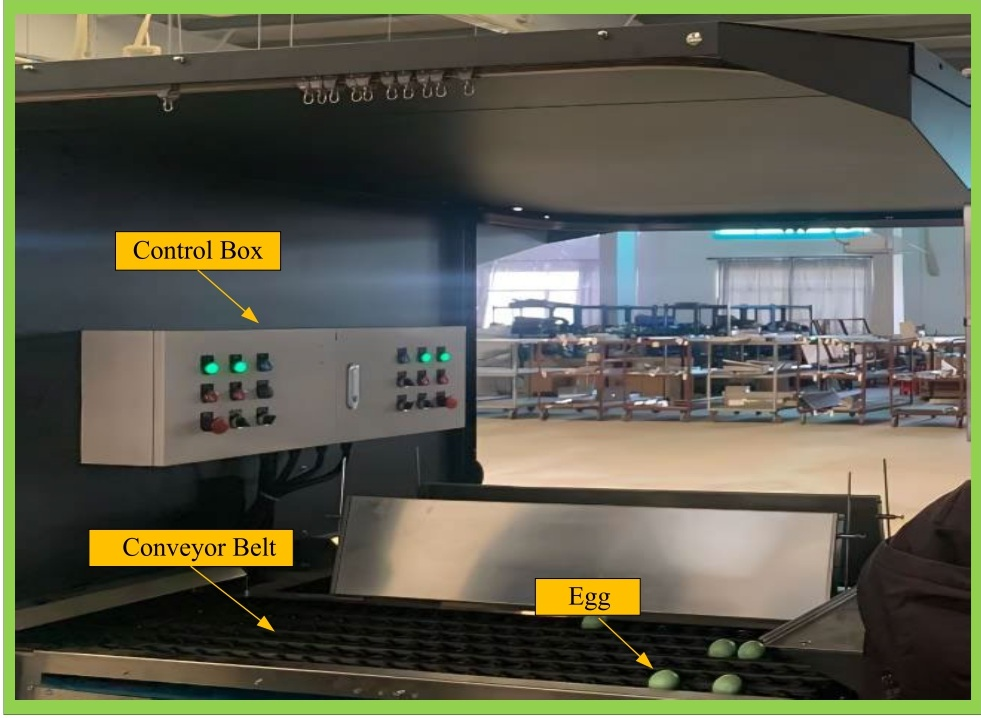
\includegraphics[width=0.62\textwidth]{figure1_egg_conveying_device.jpg}
    \caption{Multi-channel egg conveying device with parallel transport tracks and rotating rollers}
    \label{fig:conveying_device}
\end{figure}

\begin{figure}[H]
    \centering
    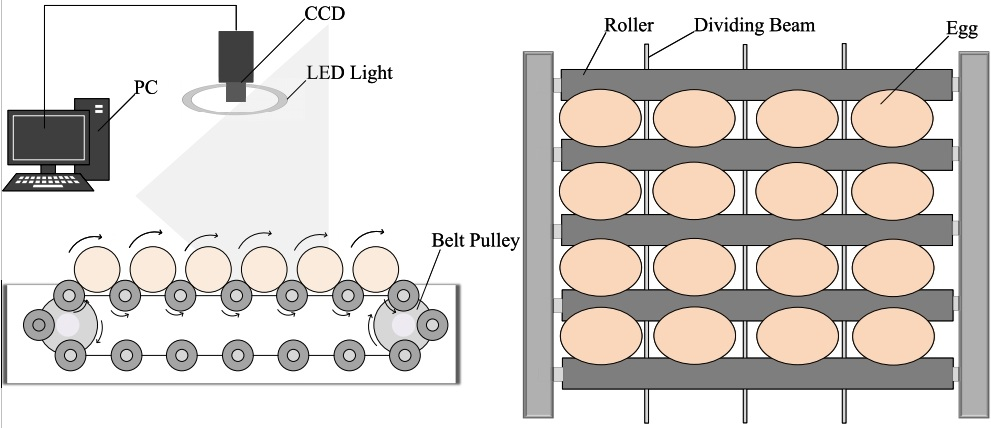
\includegraphics[width=0.62\textwidth]{figure2_machine_vision_system.jpg}
    \caption{Machine vision system layout illustrating the overhead CCD camera, LED diffuse lighting box, processing unit and roller conveyor}
    \label{fig:vision_system}
\end{figure}

The conveying device features six parallel transport channels driven by an industrial motor, with each channel carrying 60 eggs per minute for a total system throughput of 360 eggs per minute. The conveying bed consists of cylindrical rubber rollers. As the conveyor chain translates linearly forward, stationary lower guide rails force the rollers to rotate around their central axes. Consequently, eggs supported between rollers perform synchronized linear translation and continuous 360-degree axial rotation. The transit speed is calibrated so that every egg completes at least one full 360-degree rotation while traversing the camera's field of view.

The overhead industrial CCD color camera is mounted with its optical axis perpendicular to the egg motion plane, eliminating perspective distortion across all six channels. A diffuse white LED lighting box encloses the inspection zone, delivering uniform shadowless illumination that eliminates specular reflection highlights on the curved glossy shells.

\section{Industrial Dataset Acquisition and Annotation}

To ensure generalization under real-world factory conditions, dynamic video frames of unwashed chicken eggs were captured on the sorting line at Guangzhou Suiping Enterprise Co., Ltd. The collection yielded 628 raw images containing intact and cracked eggs across diverse positions, natural backgrounds and ambient lighting levels. Cracked eggs were deliberately included to maintain balanced positive and negative samples.

Using LabelImg, domain experts annotated images across three distinct categories:
\begin{itemize}
    \item \textbf{Category 1 (Intact Egg):} Bounding box enclosing the normal, undamaged egg body.
    \item \textbf{Category 2 (Cracked Egg):} Bounding box enclosing an egg body displaying shell rupture.
    \item \textbf{Category 3 (Crack Region):} Bounding box tightly fitted around the localized fracture zone.
\end{itemize}

Figure~\ref{fig:classification_categories} illustrates these three classification categories.

\begin{figure}[H]
    \centering
    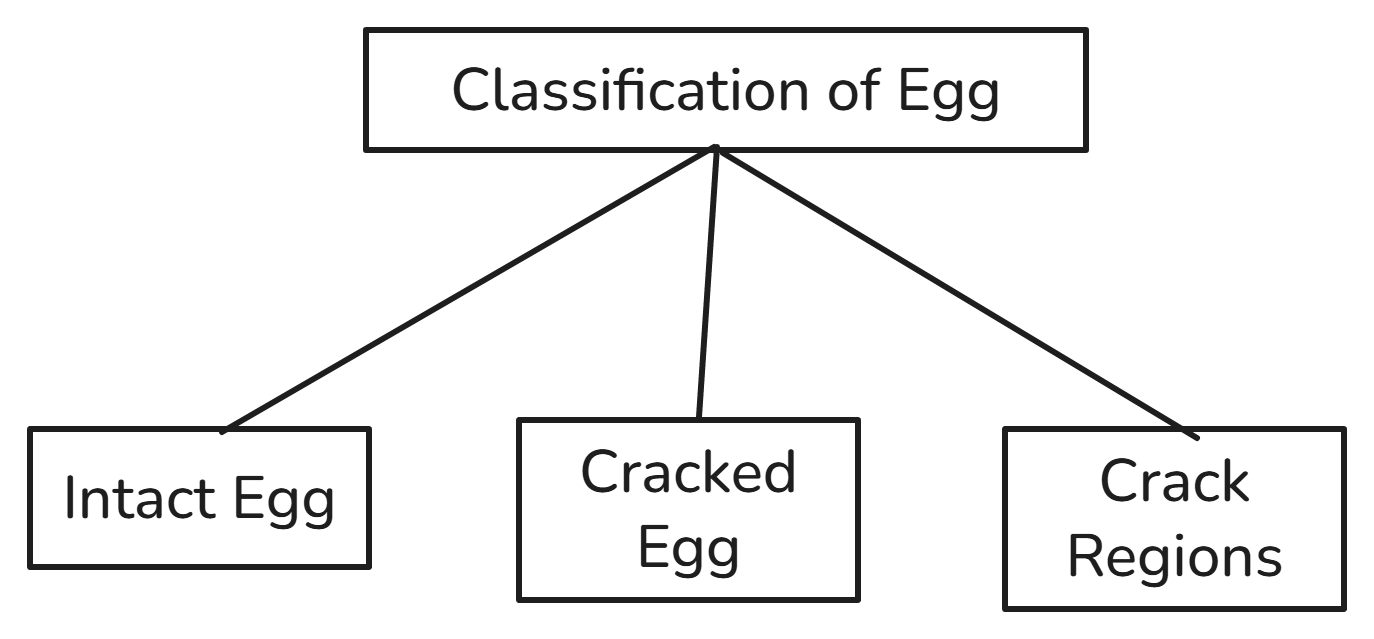
\includegraphics[width=0.75\textwidth]{classificationCategories.png}
    \caption{Visual illustration of triple classification granularity: Intact Egg, Cracked Egg and Crack Region}
    \label{fig:classification_categories}
\end{figure}

The annotated dataset was partitioned into training (377 images), validation (126 images) and test (125 images) sets in a 6:2:2 ratio. Random cropping and horizontal/vertical flipping (50\% probability) expanded the training set to 2,972 images. The total dataset comprises 3,222 images containing 7,611 intact eggs, 2,711 cracked eggs and 2,935 localized crack areas. Table~\ref{tab:dataset_distribution} details the composition.

\begin{table}[H]
\centering
\caption{Dataset composition across partitions and defect categories}
\label{tab:dataset_distribution}
\vspace{0.2cm}
\setlength{\tabcolsep}{6pt}
\renewcommand{\arraystretch}{1.15}
\small
\begin{tabular}{lcccc}
\toprule
\textbf{Partition} & \textbf{Images} & \textbf{Intact Eggs (Cat 1)} & \textbf{Cracked Eggs (Cat 2)} & \textbf{Crack Regions (Cat 3)} \\
\midrule
Training Set & 2,972 & 7,015 & 2,501 & 2,708 \\
Validation Set & 126 & 298 & 105 & 114 \\
Test Set & 125 & 298 & 105 & 113 \\
\midrule
\textbf{Total} & \textbf{3,222} & \textbf{7,611} & \textbf{2,711} & \textbf{2,935} \\
\bottomrule
\end{tabular}
\end{table}

\section{Improved YOLOv8 Network Architecture}

To detect microscopic, tortuous hairline cracks on unwashed eggs, four structural modifications were introduced to baseline YOLOv8: embedding DCNv2 into the backbone, replacing PANet with BiFPN, adding a P2 small target detection head and adopting WIoUv2 dynamic loss. Figure~\ref{fig:yolov8_arch} displays the complete network pipeline.

\begin{figure}[H]
    \centering
    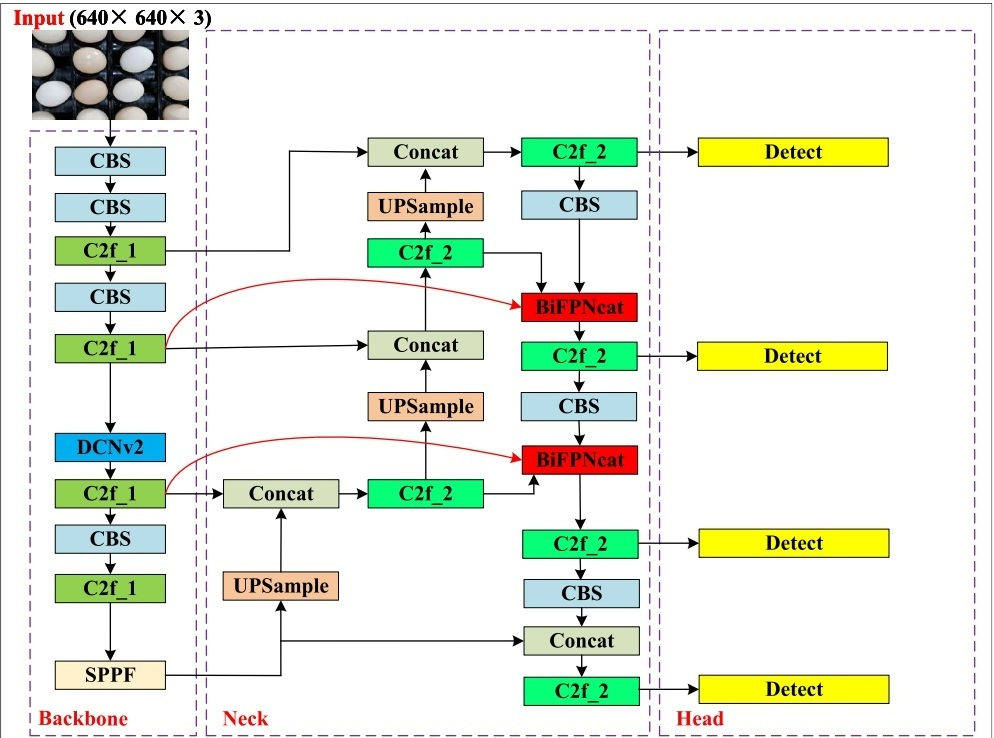
\includegraphics[width=0.88\textwidth]{figure3_improved_yolov8_architecture_1.jpg}
    \caption{Improved YOLOv8 network architecture pipeline for cracked egg detection}
    \label{fig:yolov8_arch}
\end{figure}

\subsection{Backbone Enhancement with DCNv2}

Standard convolutional layers in the YOLOv8 backbone utilize rigid $3 \times 3$ square kernels that dilute crack features with healthy shell background pixels. Standard convolutions in deep backbone layers are replaced with Deformable Convolution v2 (DCNv2). Figure~\ref{fig:dcnv2_sampling} compares normal convolution, DCNv1 and DCNv2 sampling strategies.

\begin{figure}[H]
    \centering
    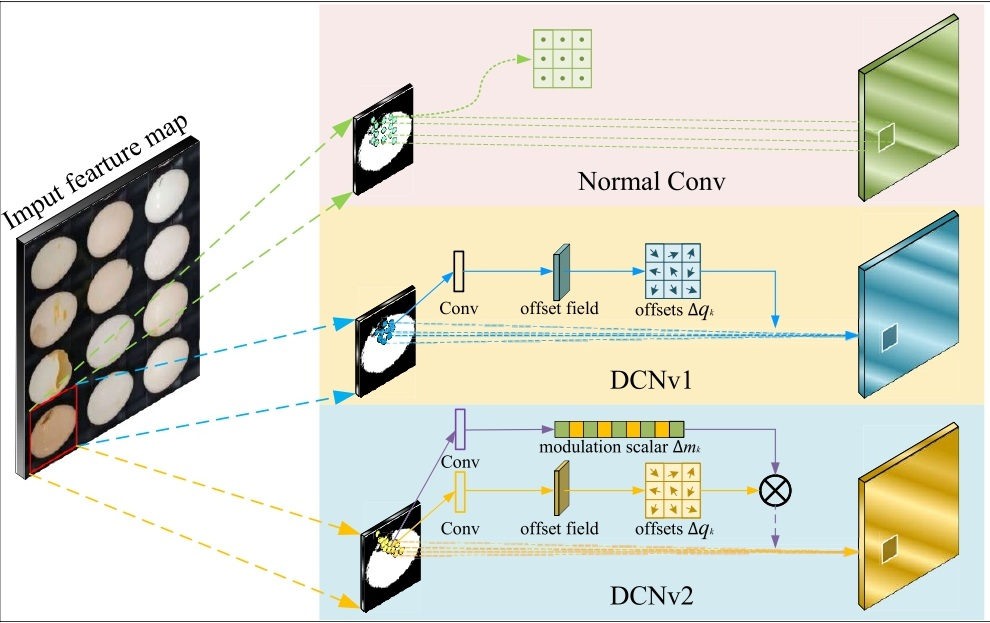
\includegraphics[width=0.72\textwidth]{figure4_dcnv2_sampling_comparison.jpg}
    \caption{Sampling grid comparison of Normal Conv, DCNv1 and DCNv2}
    \label{fig:dcnv2_sampling}
\end{figure}

DCNv2 adds learnable 2D spatial offsets $\Delta q_k$ and modulation scalars $\Delta m_k \in [0, 1]$:
\begin{equation}
Y(q) = \sum_{k=1}^{K} w_k X(q + q_k + \Delta q_k) \Delta m_k
\end{equation}
This allows receptive fields to stretch along winding fracture contours while suppressing non-crack shell textures.

\subsection{BiFPN Multi-Scale Feature Fusion}

The default PANet neck in YOLOv8 treats all input scales equally. BiFPN replaces PANet by eliminating single-edge nodes, introducing cross-scale residual skip connections and applying fast normalized weighted fusion:
\begin{equation}
O = \sum_{i} \frac{w_i}{\epsilon + \sum_{j} w_j} \cdot I_i
\end{equation}
Figure~\ref{fig:bifpn_structure} compares FPN, PANet and BiFPN topologies. BiFPN dynamically balances shallow spatial details with deep semantics, improving resilience to lighting shifts.

\begin{figure}[H]
    \centering
    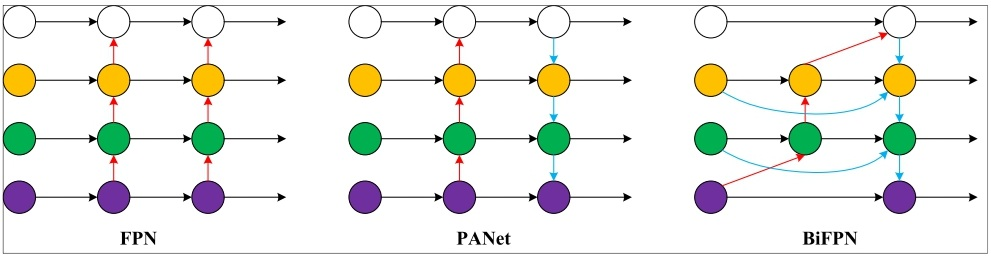
\includegraphics[width=0.78\textwidth]{figure5_fpn_panet_bifpn_structure.jpg}
    \caption{Structural comparison of FPN, PANet and BiFPN multi-scale fusion}
    \label{fig:bifpn_structure}
\end{figure}

\subsection{Small Target Detection Head and WIoUv2 Loss}

The baseline P3 detection head ($80 \times 80$) possesses an $8 \times 8$ pixel receptive field, causing sub-8-pixel cracks to disappear during downsampling. A 4th detection head operating on a $160 \times 160$ feature map (P2, stride 4, $4 \times 4$ px receptive field) is added to preserve early spatial gradients.

To balance gradients across bounding box candidates, Wise-IoU v2 (WIoUv2) loss is adopted:
\begin{equation}
L_{\text{WIoUv2}} = \left(\frac{L_{\text{IoU}}}{\overline{L_{\text{IoU}}}}\right)^\gamma L_{\text{WIoUv1}}, \quad \gamma > 0
\end{equation}
WIoUv2 reduces penalty gradients on extreme low-quality outliers while focusing updates on high-potential candidates.

\section{Dual Verification Decision-Making Mechanism}

Under the triple classification granularity scheme, the detector simultaneously outputs bounding box predictions for Category 1 ($C_1$), Category 2 ($C_2$) and Category 3 ($C_3$). The dual verification decision rule identifies an egg as damaged if:
\begin{equation}
\text{Status} = \begin{cases}
\text{Cracked (Reject)} & \text{if } (C_2 \ge 1) \lor (C_3 \ge 1) \\
\text{Intact (Accept)} & \text{if } (C_1 \ge 1) \land (C_2 = 0) \land (C_3 = 0)
\end{cases}
\end{equation}

A defective egg is missed only if both detection branches fail simultaneously:
\begin{equation}
P(\text{Miss}_{\text{Overall}}) = P(\text{Miss}_{\text{Egg}}) \times P(\text{Miss}_{\text{Region}})
\end{equation}
Because both individual miss rates are small percentages, their compound product drastically lowers missed defect escapes.

\section{Model Training Workflow}

Figure~\ref{fig:training_schematic} illustrates the end-to-end model training, validation and deployment workflow.

\begin{figure}[H]
    \centering
    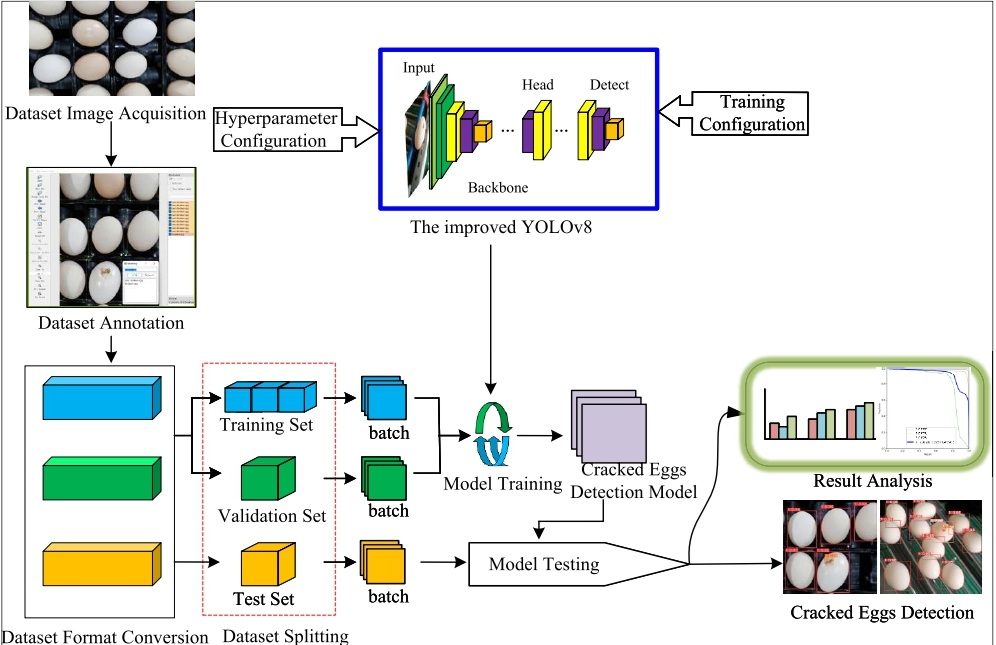
\includegraphics[width=0.78\textwidth]{figure6_training_schematic.jpg}
    \caption{Flowchart of data acquisition, model training, validation and factory deployment}
    \label{fig:training_schematic}
\end{figure}

Training was conducted on an Intel Core i5-10400F CPU (2.9 GHz) with an NVIDIA GeForce RTX 3060 GPU (12 GB VRAM) and 32 GB RAM under Windows 10, Python 3.8 and PyTorch 1.13.1. Training parameters: input size $640 \times 640$, batch size 16, SGD optimizer (momentum 0.937, weight decay 0.0005), initial learning rate 0.01, random seed 42 and exactly 300 epochs trained from scratch without pre-trained weights.
%=========================================================
% CHAPTER 5
%=========================================================

\chapter{Results and Discussion}

\section{Experimental Setup and Evaluation Metrics}

The computational environment and hyperparameters utilized for offline training and evaluation are summarized in Table~\ref{tab:hardware_software}.

\begin{table}[H]
\centering
\caption{Computational hardware specifications and software environment}
\label{tab:hardware_software}
\vspace{0.2cm}
\setlength{\tabcolsep}{8pt}
\renewcommand{\arraystretch}{1.15}
\small
\begin{tabular}{ll}
\toprule
\textbf{Component / Parameter} & \textbf{Specification / Value} \\
\midrule
Operating System & Microsoft Windows 10 (64-bit) \\
Central Processing Unit (CPU) & Intel Core i5-10400F @ 2.90 GHz \\
Graphics Processing Unit (GPU) & NVIDIA GeForce RTX 3060 (12 GB VRAM) \\
System Memory (RAM) & 32 GB DDR4 (3200 MHz) \\
Framework and Language & PyTorch 1.13.1, CUDA 11.6, Python 3.8 \\
Image Resolution & $640 \times 640$ pixels \\
Training Epochs and Batch Size & 300 epochs, batch size 16 \\
Optimizer and Initial LR & SGD (momentum: 0.937), initial lr: 0.01 \\
\bottomrule
\end{tabular}
\end{table}

Standard evaluation metrics are defined as follows:
\begin{equation}
\text{Precision} = \frac{\text{TP}}{\text{TP} + \text{FP}}, \quad \text{Recall} = \frac{\text{TP}}{\text{TP} + \text{FN}}
\end{equation}
\begin{equation}
\text{mAP@0.5} = \frac{1}{N_c} \sum_{i=1}^{N_c} \text{AP}_i, \quad \text{FNR} = \frac{\text{FN}}{\text{TP} + \text{FN}}, \quad \text{FPR} = \frac{\text{FP}}{\text{FP} + \text{TN}}
\end{equation}
where TP, FP, TN and FN denote true positives, false positives, true negatives and false negatives respectively and FPS measures frames processed per second.

\section{Ablation Study and Analysis of Proposed Modules}

To quantify the individual contributions of DCNv2, BiFPN, WIoU and the P2 small target detection head, eight ablation variants were evaluated. Table~\ref{tab:ablation_results} reports test dataset performance.

\begin{table}[H]
\centering
\caption{Ablation experiment results on test dataset}
\label{tab:ablation_results}
\vspace{0.2cm}
\setlength{\tabcolsep}{6pt}
\renewcommand{\arraystretch}{1.15}
\small
\begin{tabular}{cccc|ccc}
\toprule
\textbf{DCNv2} & \textbf{BiFPN} & \textbf{WIoU} & \textbf{Small Target Head} & \textbf{Precision (\%)} & \textbf{Recall (\%)} & \textbf{mAP@0.5 (\%)} \\
\midrule
- & - & - & - & 92.2 & 85.3 & 87.7 \\
- & - & \checkmark & - & 90.6 & 87.4 & 90.3 \\
- & \checkmark & - & - & 89.8 & 83.8 & 88.2 \\
- & - & - & \checkmark & 93.8 & 90.3 & 93.0 \\
\checkmark & - & \checkmark & - & 93.1 & 89.4 & 92.1 \\
- & \checkmark & \checkmark & - & 92.6 & 89.5 & 92.2 \\
\checkmark & \checkmark & \checkmark & - & 93.8 & 89.9 & 92.6 \\
\checkmark & \checkmark & \checkmark & \checkmark & \textbf{94.1} & \textbf{90.0} & \textbf{92.9} \\
\bottomrule
\end{tabular}
\end{table}

Key observations from the ablation study:
\begin{enumerate}[label=\arabic*.]
    \item Replacing CIoU with WIoU boosted mAP from 87.7\% to 90.3\% (+2.6\%), demonstrating the value of dynamic gradient weighting.
    \item The P2 small target head yielded the largest single-module improvement (+5.3\% mAP), preserving high-frequency micro-crack edges.
    \item The full four-component ensemble achieved the highest precision (94.1\%) and balanced recall (90.0\%) with 92.9\% mAP (+5.2\% over baseline), proving that DCNv2 and BiFPN provide crucial robustness against irregular crack shapes and illumination variations.
\end{enumerate}

\section{Model Complexity and Benchmark Comparison}

Table~\ref{tab:model_complexity} compares model complexity between baseline YOLOv8 and the improved model. The structural enhancements introduce only +2.7\% parameters, +9.3\% FLOPs and +1.5 MB in model size.

\begin{table}[H]
\centering
\caption{Model complexity and computational footprint comparison}
\label{tab:model_complexity}
\vspace{0.2cm}
\setlength{\tabcolsep}{10pt}
\renewcommand{\arraystretch}{1.15}
\small
\begin{tabular}{lccc}
\toprule
\textbf{Model Architecture} & \textbf{Parameters} & \textbf{FLOPs (G)} & \textbf{Model Size (MB)} \\
\midrule
Baseline YOLOv8 & $2.59 \times 10^7$ & 79.1 & 49.6 \\
Proposed Improved YOLOv8 & $2.66 \times 10^7$ & 86.5 & 51.1 \\
\midrule
\textbf{Relative Increase} & \textbf{+2.7\%} & \textbf{+9.3\%} & \textbf{+3.0\%} \\
\bottomrule
\end{tabular}
\end{table}

Table~\ref{tab:benchmark_comparison} compares the proposed model against mainstream detectors on the unwashed egg dataset. The proposed model outperforms Faster R-CNN by 14.8\% mAP, YOLOv5 by 7.7\% mAP, baseline YOLOv8 by 5.2\% mAP and YOLOv11 by 5.6\% mAP. At 45 FPS, its throughput comfortably satisfies the $\ge 30$ FPS industrial standard.

\begin{table}[H]
\centering
\caption{Comparative performance benchmark across mainstream detectors}
\label{tab:benchmark_comparison}
\vspace{0.2cm}
\setlength{\tabcolsep}{8pt}
\renewcommand{\arraystretch}{1.15}
\small
\begin{tabular}{lcccc}
\toprule
\textbf{Object Detection Model} & \textbf{Precision (\%)} & \textbf{Recall (\%)} & \textbf{mAP@0.5 (\%)} & \textbf{Speed (FPS)} \\
\midrule
Faster R-CNN (ResNet50) & 68.4 & 80.7 & 78.1 & 17 \\
YOLOv5 & 86.9 & 81.1 & 85.2 & 58 \\
YOLOv8 (Baseline) & 92.2 & 85.3 & 87.7 & 52 \\
YOLOv11 & 92.7 & 84.3 & 87.3 & 47 \\
\textbf{Proposed Improved YOLOv8} & \textbf{94.1} & \textbf{90.0} & \textbf{92.9} & \textbf{45} \\
\bottomrule
\end{tabular}
\end{table}

\section{Precision-Recall Dynamics and Visual Results}

Figure~\ref{fig:pr_curves} displays Precision-Recall curves before and after model improvement, showing expanded area under the curve across all three categories. Figure~\ref{fig:visual_detection} shows side-by-side visual detection comparisons: baseline YOLOv8 misses faint cracks and misclassifies surface dirt, whereas the improved model accurately localizes both the cracked egg body and tight damage regions.

\begin{figure}[H]
    \centering
    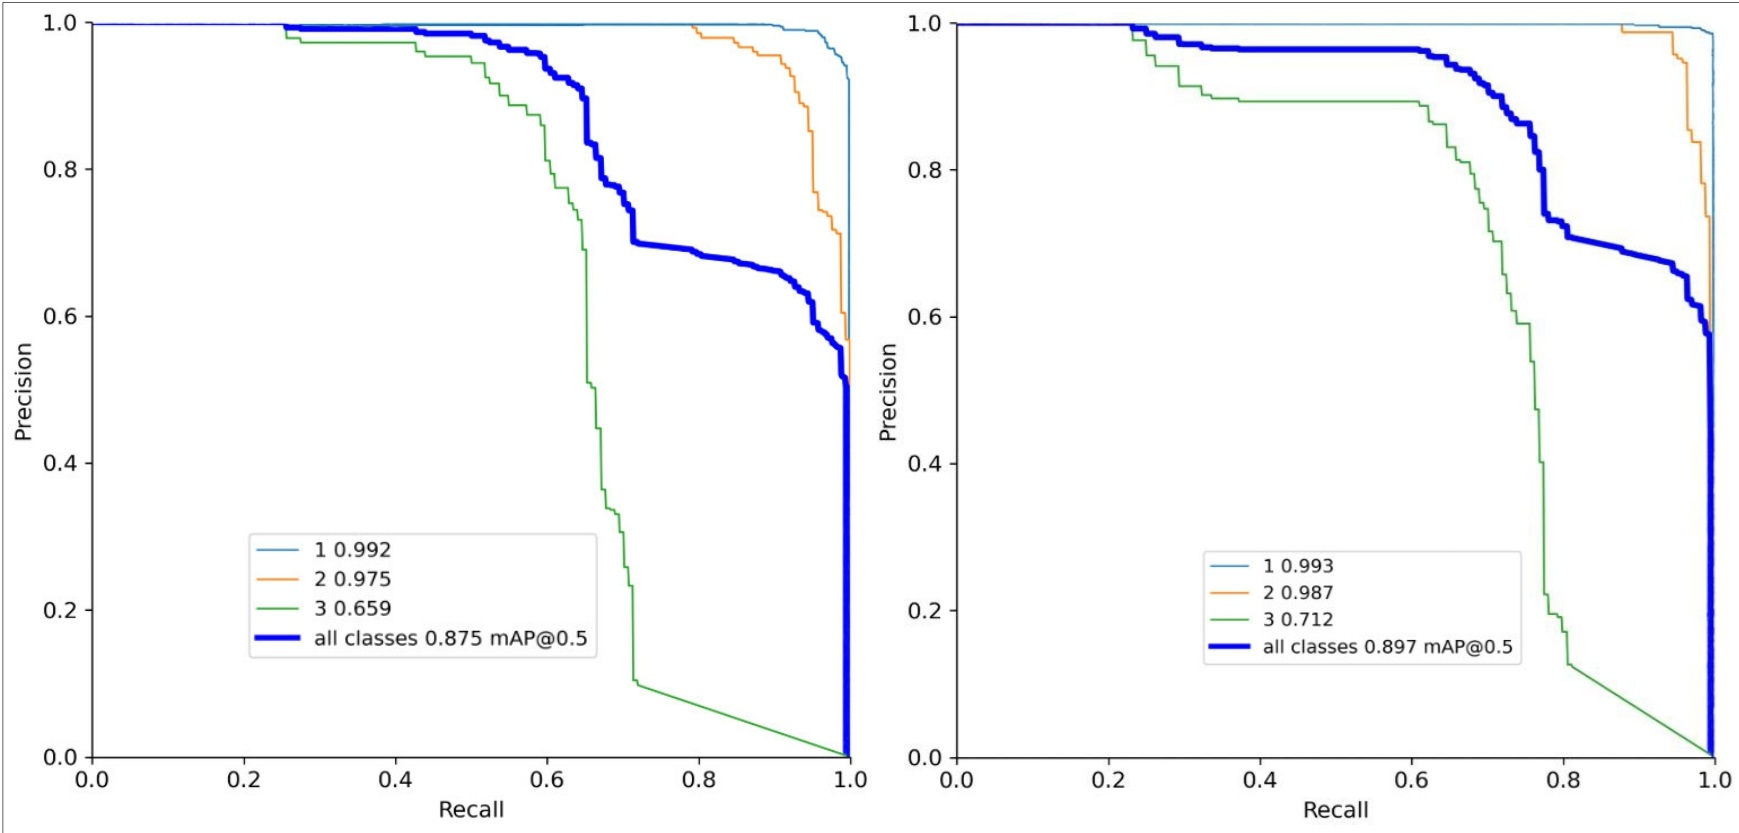
\includegraphics[width=0.75\textwidth]{figure8_pr_curves_comparison.jpg}
    \caption{Precision-Recall (P-R) curves before and after model improvement}
    \label{fig:pr_curves}
\end{figure}

\begin{figure}[H]
    \centering
    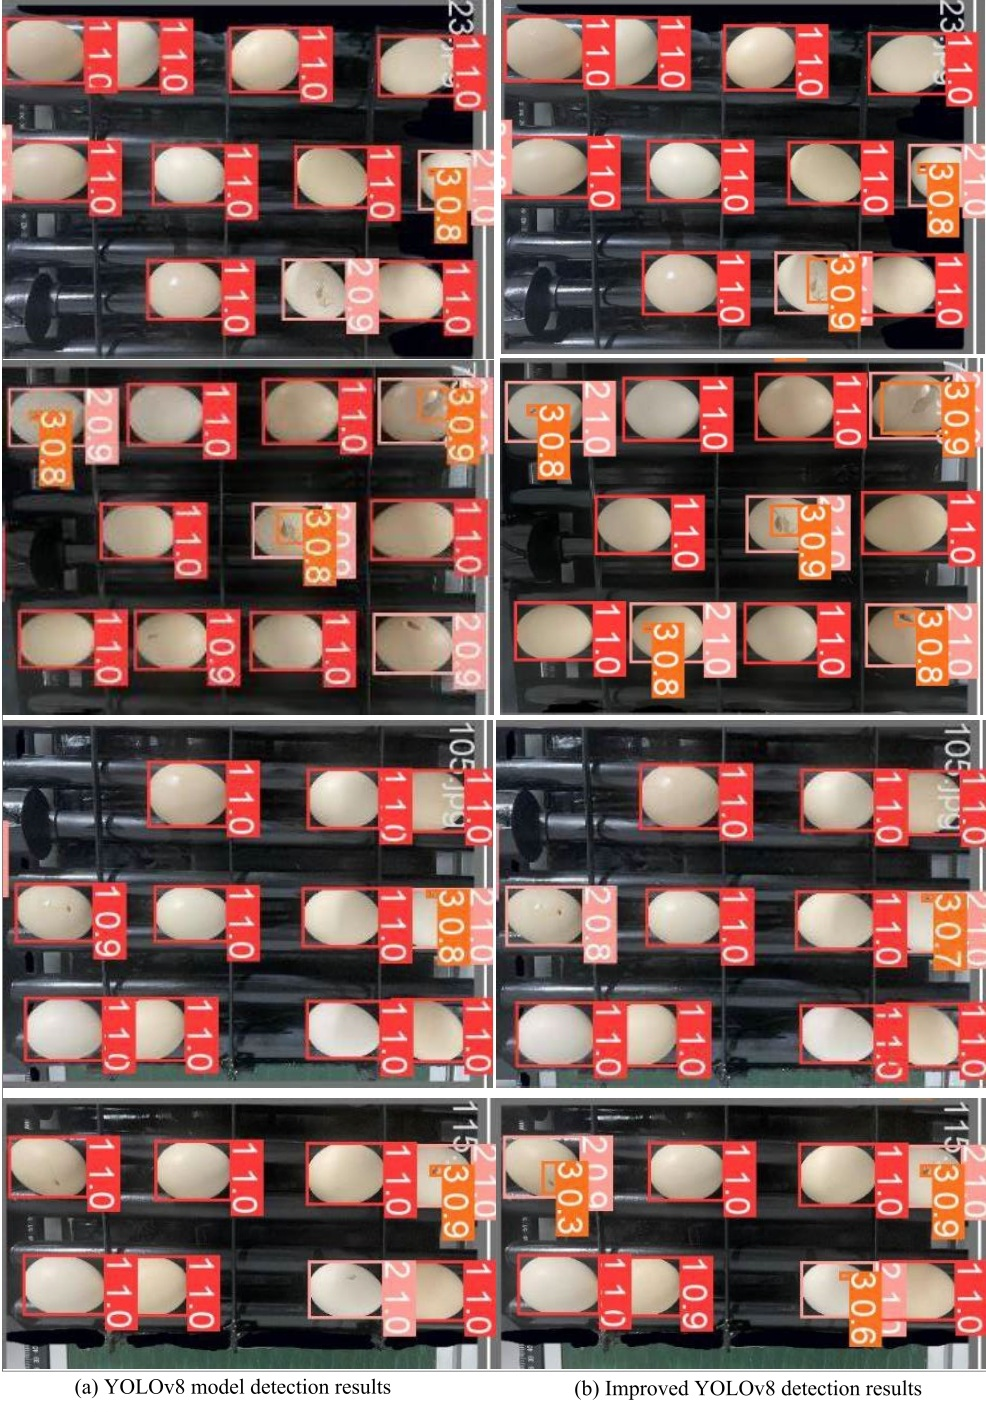
\includegraphics[width=0.78\textwidth]{figure9_detection_effects_comparison.jpg}
    \caption{Visual detection comparison on test frames: Left shows baseline YOLOv8, Right shows proposed improved YOLOv8}
    \label{fig:visual_detection}
\end{figure}

\section{Industrial Production Line Online Testing}

The system was deployed on the physical conveyor line at Guangzhou Suiping Enterprise Co., Ltd., as shown in Figure~\ref{fig:online_deployment}. Detection accuracy was benchmarked across 106 production video frames, with error rates presented in Table~\ref{tab:online_inspection_errors}.

\begin{figure}[H]
    \centering
    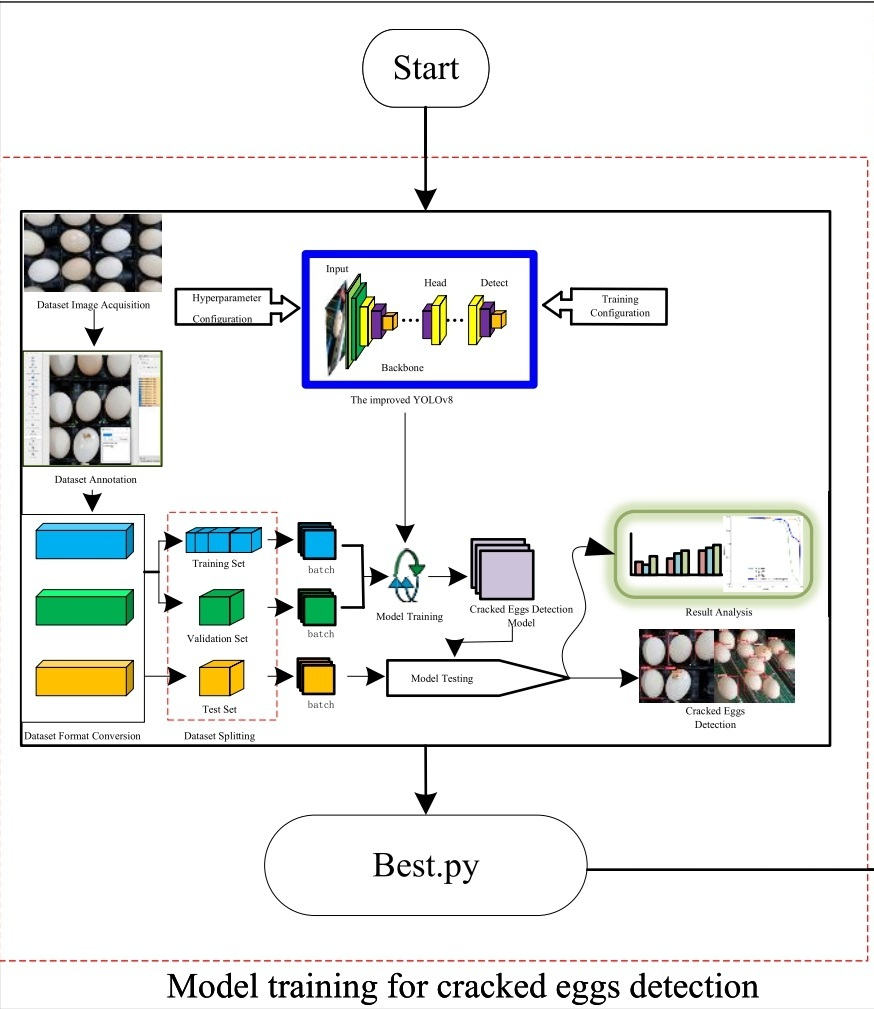
\includegraphics[width=0.72\textwidth]{figure7_online_deployment_testing_1.jpg}
    \caption{Online deployment and testing on the industrial egg conveyor line}
    \label{fig:online_deployment}
\end{figure}

\begin{table}[H]
\centering
\caption{Online factory inspection error rates across 106 production video frames}
\label{tab:online_inspection_errors}
\vspace{0.2cm}
\setlength{\tabcolsep}{6pt}
\renewcommand{\arraystretch}{1.2}
\small
\begin{tabular}{l|cc|cc}
\toprule
\textbf{Classification Category} & \multicolumn{2}{c|}{\textbf{Baseline YOLOv8}} & \multicolumn{2}{c}{\textbf{Proposed Improved YOLOv8}} \\
& \textbf{FNR (\%)} & \textbf{FPR (\%)} & \textbf{FNR (\%)} & \textbf{FPR (\%)} \\
\midrule
Class 1: Intact Egg & 1.26 & 4.00 & \textbf{0.46} & \textbf{2.18} \\
Class 2: Cracked Egg & 10.17 & 3.20 & \textbf{5.52} & \textbf{1.16} \\
Class 3: Damaged Area & 22.97 & 0.87 & \textbf{19.19} & \textbf{0.58} \\
\midrule
\textbf{Compound Dual Verification FNR} & \multicolumn{2}{c|}{$10.17\% \times 22.97\% = 2.34\%$} & \multicolumn{2}{c}{$\mathbf{5.52\% \times 19.19\% = 1.06\%}$} \\
\bottomrule
\end{tabular}
\end{table}

Key factory findings:
\begin{itemize}
    \item Intact egg false alarm rate (FPR) dropped from 4.00\% to 2.18\%, saving marketable eggs.
    \item Cracked egg miss rate (FNR) was reduced by nearly half from 10.17\% to 5.52\%.
    \item Compound broken egg miss rate fell to just 1.06\%, ensuring industrial reliability.
\end{itemize}

Figure~\ref{fig:production_detection} shows live conveyor tracking with rotating eggs and Figure~\ref{fig:online_speed} confirms consistent inference speed hovering stably at 45 FPS across 400 continuous frames.

\begin{figure}[H]
    \centering
    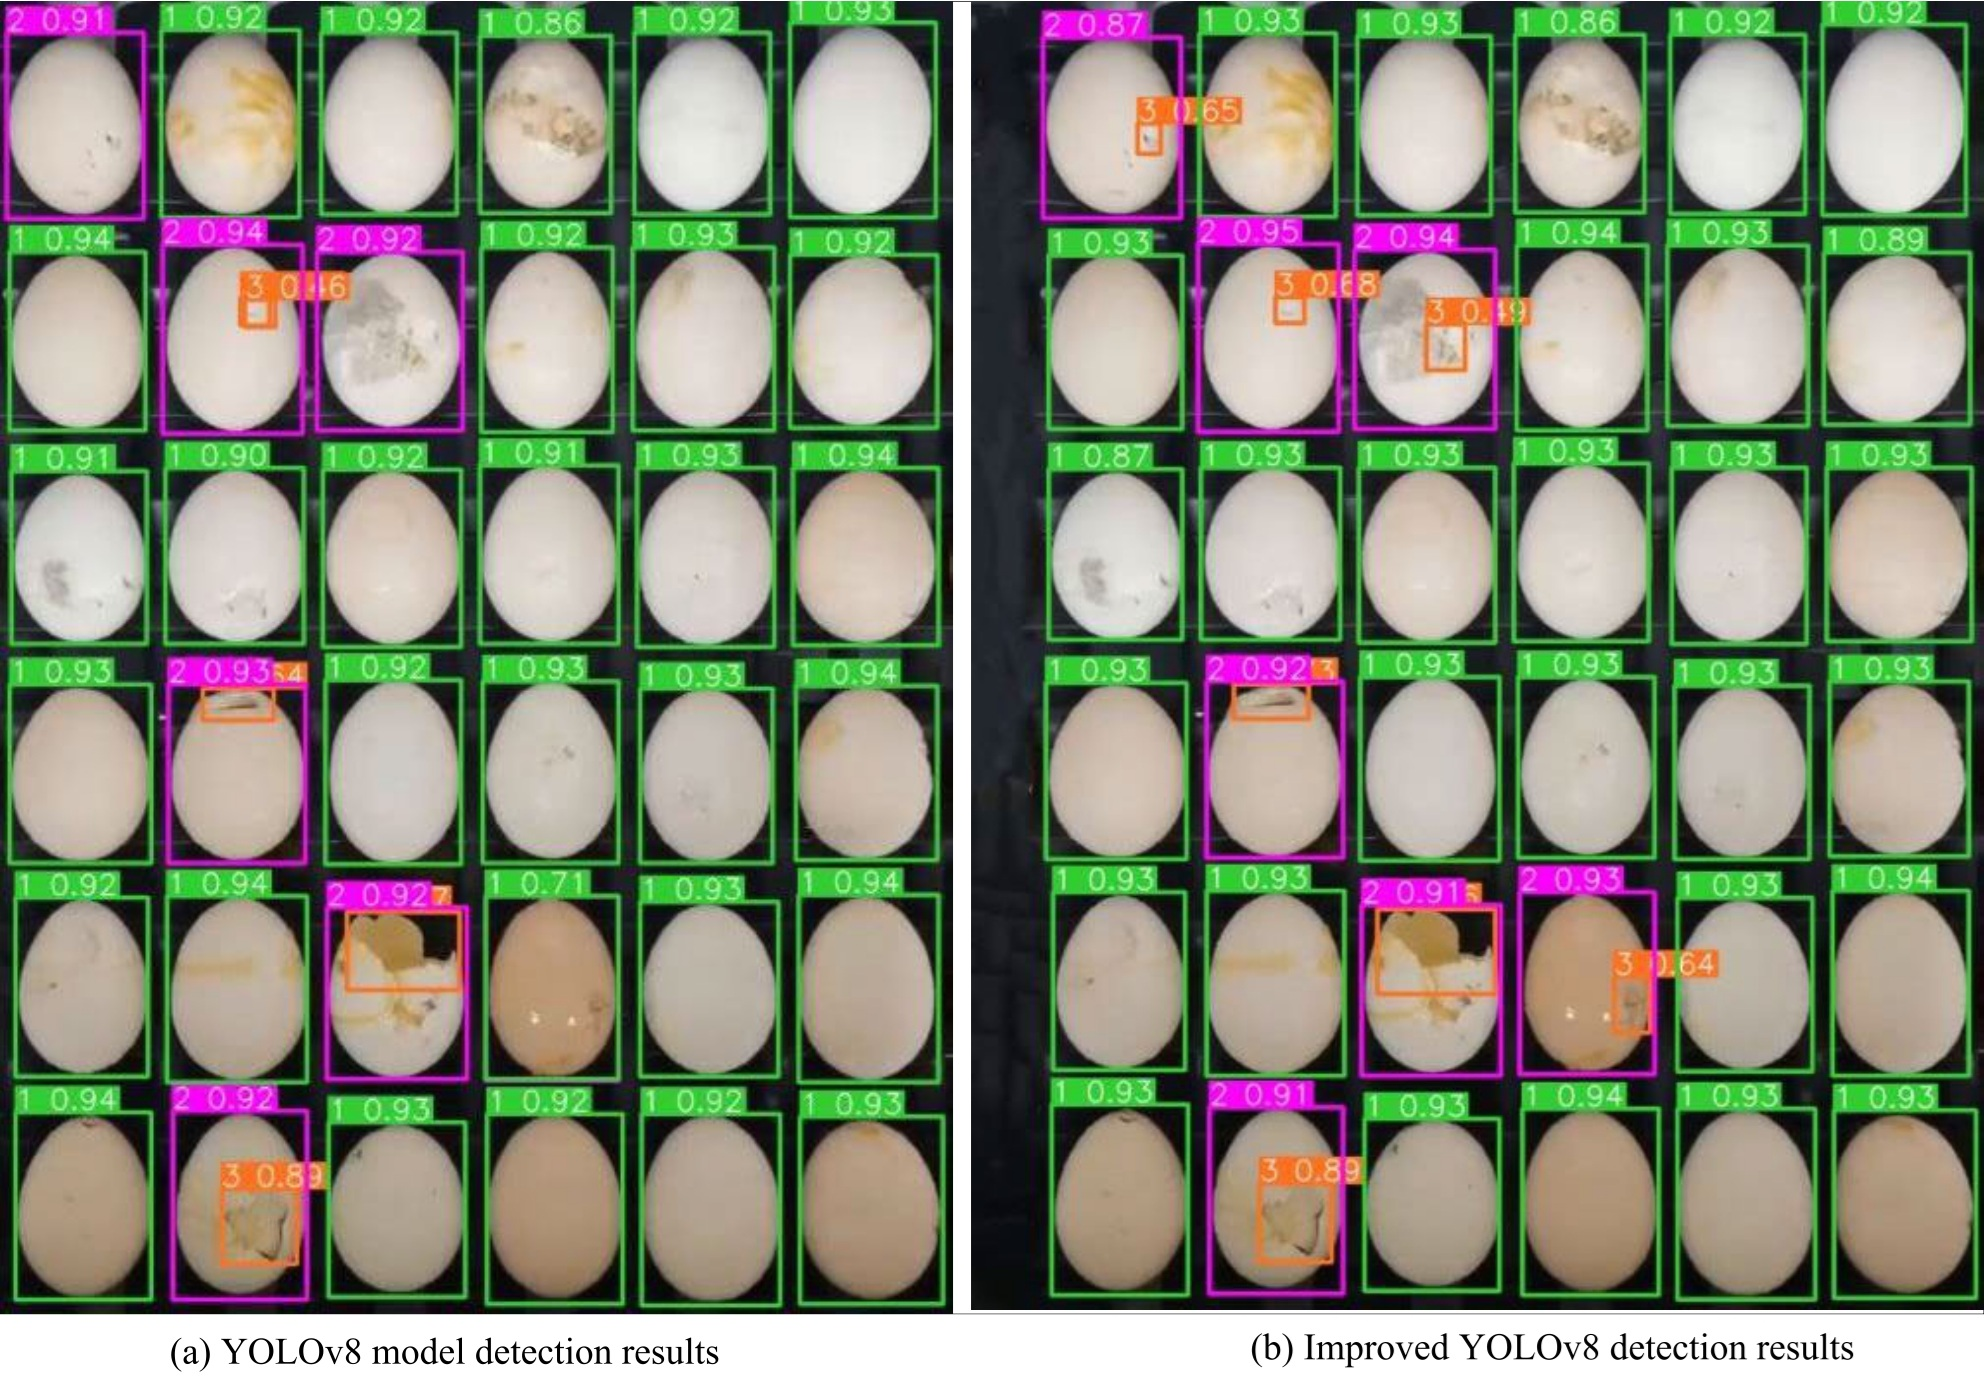
\includegraphics[width=0.78\textwidth]{figure10_production_line_detection.jpg}
    \caption{Visual detection results on active industrial conveyor with rotating eggs}
    \label{fig:production_detection}
\end{figure}

\begin{figure}[H]
    \centering
    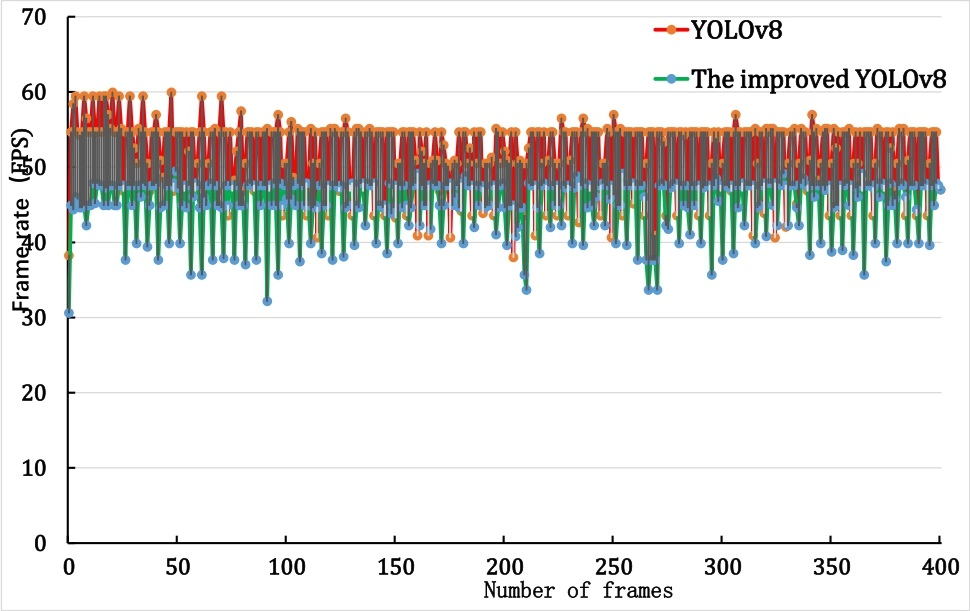
\includegraphics[width=0.75\textwidth]{figure11_online_detection_speed.jpg}
    \caption{Online detection speed stability curve across 400 continuous frames at 45 FPS}
    \label{fig:online_speed}
\end{figure}

\section{Discussion of Operational Findings and Edge Cases}

The slight speed reduction from 52 FPS to 45 FPS (-14.5\%) provided a +5.2\% mAP gain while maintaining comfortable real-time margin over the 30 FPS line rate. Combining DCNv2 with triple granularity decoupled true crack edges from manure and dust on unwashed eggs. While plain shells (white eggs and duck eggs) exhibited high contrast, fine reticular spider-web cracks (widths $< 0.03$ mm) remain the primary edge-case challenge under diffuse lighting.
%=========================================================
% CHAPTER 6
%=========================================================

\chapter{Applications and Practical Implementation}

\section{Industrial Egg Grading and Packaging Lines}

In commercial poultry packaging facilities processing 30,000 to 180,000 eggs per hour (e.g., Kyowa, Moba and Sanovo grading machines), the improved YOLOv8 vision system serves as an automated quality gateway installed prior to washing tanks. Detecting and ejecting cracked eggs before washing prevents wash water from being drawn into egg interiors via capillary suction, protecting sanitation and preventing batch-wide bacterial cross-contamination.

\section{Real-Time Online Rejection Mechanisms}

The vision system interfaces with downstream programmable logic controllers (PLCs) through rotary encoder synchronization. Optical shaft encoders track the millimeter displacement of individual roller pockets. When a defect is detected, high-speed solenoid pneumatic air-jet valves discharge a calibrated compressed air pulse (under 20 ms) that lifts the defective egg into a collection chute, achieving reliable non-contact rejection at line speeds.

\section{Embedded Edge Computing Deployment}

With a compact footprint of 51.1 MB and 86.5 G FLOPs, the improved model can be deployed on edge hardware such as the NVIDIA Jetson AGX Orin. Utilizing TensorRT FP16 quantization accelerates inference latency to under 12 milliseconds per frame, enabling direct installation within ruggedized factory control cabinets.

\section{Environmental Maintenance and Operational Protocols}

Demanding poultry farm environments require active maintenance measures:
\begin{itemize}
    \item \textbf{Positive-Pressure Air Knives:} Continuous laminar airflow over optical lens surfaces prevents airborne feather dust and moisture droplets from settling on glass apertures.
    \item \textbf{LED Thermal Regulation:} Thermostatically controlled cooling fans prevent LED color temperature drift across seasonal shifts.
    \item \textbf{Illumination Self-Calibration:} Periodic reference checks on empty white rollers automatically adjust camera exposure times to compensate for diode aging.
\end{itemize}

\section{Economic Benefits and Food Safety Assurance}

Deploying automated crack detection replaces two to four manual candling operators per shift, substantially lowering labor payrolls. Lowering the intact egg false alarm rate to 2.18\% preserves 1.82\% of marketable eggs, saving over 1,820 eggs daily in a 100,000 egg/day plant. Furthermore, reducing broken egg escapes to 1.06\% provides robust protection against \textit{Salmonella} outbreaks, protecting brand integrity and eliminating emergency shutdowns caused by leaking yolk fouling conveyor machinery.
%=========================================================
% CHAPTER 7
%=========================================================

\chapter{Conclusion and Future Scope}

\section{Conclusion}

This seminar presented a comprehensive investigation of an industrial-grade, real-time cracked egg detection system combining an improved YOLOv8 architecture, multi-channel rotational conveyance and dual verification with triple classification granularity.

The key achievements of the study are:
\begin{enumerate}[label=\arabic*.]
    \item A six-channel roller conveyor imparting synchronized translation and continuous axial rotation eliminated shell inspection blind spots.
    \item Triple classification granularity (Intact Egg, Cracked Egg and Crack Region) provided multi-scale supervision, while redundant dual verification lowered compound miss rates to 1.06\%.
    \item Architectural optimizations (DCNv2, BiFPN, P2 small target head and WIoUv2 loss) achieved an mAP@0.5 of 92.9\% and 94.1\% precision, outperforming Faster R-CNN, YOLOv5 and YOLOv11 with negligible overhead.
    \item Live industrial deployment sustained 45 FPS across 400 frames, reducing intact egg false alarms to 2.18\% and satisfying factory grading criteria.
\end{enumerate}

\section{Practical Limitations}

Current limitations include vulnerability to ultra-fine reticular spider-web cracks ($< 0.03$ mm) that produce minimal shadow relief under diffuse top-down lighting and restriction to exterior surface defects without internal candling for blood spots or yolk deterioration.

\section{Future Scope}

Future research directions include:
\begin{enumerate}[label=\arabic*.]
    \item \textbf{Dark-Field and Polarized Illumination:} Lateral grazing lighting to make hairline micro-cracks glow brightly against dark shell backgrounds.
    \item \textbf{Multi-Modal Vision and Spectroscopy:} Integrating NIR transmission spectroscopy for simultaneous internal freshness and shell crack inspection.
    \item \textbf{Super-Resolution Networks:} Deploying lightweight patch-level generative models to magnify subtle gradient fissures without high-cost camera upgrades.
    \item \textbf{Cross-Species Generalization:} Extending datasets to speckled quail eggs and textured duck eggs for universal poultry grading.
\end{enumerate}

%=========================================================
% REFERENCES
%=========================================================

\chapter*{References}
\addcontentsline{toc}{chapter}{References}

\begin{enumerate}[label={[\arabic*]}]

\item D. Sun, H. Wei, Y. Luo, W. Li and Y. Yu,
``Real-Time Detection Method for Cracked Eggs Based on Improved YOLOv8 and Dual Verification With Triple Classification Granularity,''
\textit{IEEE Access}, vol. 14, pp. 62322-62333, Apr. 2026, doi: 10.1109/ACCESS.2026.3686452.

\item D. Liang, P. Li, D. Liang, J. Qian and B. Li,
``Integrated detection and grading system for internal and external quality of eggs based on machine vision,''
\textit{Journal of Chinese Institute of Food Science and Technology}, vol. 20, no. 11, pp. 247-254, Nov. 2020.

\item A. Datta, B. Botta and S. Gattam,
``Damage detection on chicken eggshells using faster R-CNN,''
in \textit{Proc. ASABE Annual International Meeting}, Boston, MA, USA, Jul. 2019, p. 1244.

\item M. Turkoglu,
``Defective egg detection based on deep features and bidirectional long-short-term-memory,''
\textit{Computers and Electronics in Agriculture}, vol. 185, Jun. 2021, Art. no. 106152.

\item B. Botta, S. S. R. Gattam and A. K. Datta,
``Eggshell crack detection using deep convolutional neural networks,''
\textit{Journal of Food Engineering}, vol. 315, Feb. 2022, Art. no. 110798.

\item J. Yin, J. Kang and D. Xiao,
``Lightweight duck egg crack detection algorithm based on improved YOLOv5l,''
\textit{Transactions of the Chinese Society of Agricultural Engineering}, vol. 40, no. 1, pp. 165-173, Jan. 2024.

\item Y. Huang, Y. Luo, Y. Cao, X. Lin, H. Wei, M. Wu, X. Yang and Z. Zhao,
``Damage detection of unwashed eggs through video and deep learning,''
\textit{Foods}, vol. 12, no. 11, p. 2179, May 2023.

\item X. Zhu, H. Hu, S. Lin and J. Dai,
``Deformable ConvNets v2: More Deformable, Better Results,''
in \textit{Proc. IEEE/CVF Conference on Computer Vision and Pattern Recognition (CVPR)}, Long Beach, CA, USA, Jun. 2019, pp. 9308-9316.

\item M. Tan, R. Pang and Q. V. Le,
``EfficientDet: Scalable and Efficient Object Detection,''
in \textit{Proc. IEEE/CVF Conference on Computer Vision and Pattern Recognition (CVPR)}, Seattle, WA, USA, Jun. 2020, pp. 10778-10787.

\item Z. Tong, Y. Chen, Z. Xu and R. Yu,
``Wise-IoU: Bounding Box Regression Loss with Dynamic Focusing Mechanism,''
\textit{arXiv preprint arXiv:2301.10051}, Jan. 2023.

\item Z. Balci, I. Yabanova and A. Mert,
``An acoustic signal-to-image conversion integrated convolutional neural network model for egg crack detection,''
\textit{British Poultry Science}, vol. 67, no. 2, pp. 224-232, Mar. 2026.

\item L. Sun, S. Feng, C. Chen, X. Liu and J. Cai,
``Identification of eggshell crack for hen egg and duck egg using correlation analysis based on acoustic resonance method,''
\textit{Journal of Food Process Engineering}, vol. 43, no. 8, p. 13430, Aug. 2020.

\item A. Nasiri, M. Omid and A. Taheri-Garavand,
``An automatic sorting system for unwashed eggs using deep learning,''
\textit{Journal of Food Engineering}, vol. 283, Oct. 2020, Art. no. 110036.

\item Y. Luo, Y. Huang, Q. Wang, K. Yuan, Z. Zhao and Y. Li,
``An improved YOLOv5 model: Application to leaky eggs detection,''
\textit{LWT - Food Science and Technology}, vol. 187, Sep. 2023, Art. no. 115313.

\item J. Redmon, S. Divvala, R. Girshick and A. Farhadi,
``You only look once: Unified, real-time object detection,''
in \textit{Proc. IEEE Conference on Computer Vision and Pattern Recognition (CVPR)}, Las Vegas, NV, USA, Jun. 2016, pp. 779-788.

\end{enumerate}

\end{document}